\chapter{Background}
The FX market differs from other financial markets such as the stock market mainly by the fact that it is a partially decentralized market; there is no central trading authority. The FX market works instead with an inter-bank market and a retail market, with the inter-bank market being comprised of transactions between banks, market-makers and large institutions at typically large volumes done through central electronic brokers such as EBS and Reuters. The retail market(small/day traders) will typically interact with the banks and submit orders through the bank at the bank's given rate. The retail market generally does not have access to the same large central electronic brokers and hence must trade through the banks due to the high cost of connecting to the central exchanges and the high minimum deal sizes required to participate. Secondly, there is no market close/open, since the market runs 24 hours a day excluding weekends from 5pm EST Sunday until 4pm EST on Friday. Lastly, the FX market commonly has traders using high leverage. It is common to see 10:1 debt to equity ratios in a transaction and it is not uncommon to see 100:1 leverage ratios or even greater than this\cite{leverage}.
	
Due to the decentralized nature of the market, all of the participants do not have the same amount of information. Banks tend to have a greater access to information in the form of private order flows from their customers. Furthermore, since the banks will generally take on the role of the dealer as well as that of a trader, they often have an advantage when making speculative trades.

\section{Model Architecture}
The basic underlying architecture of the proposed model in this project will consist of three different types of agents. There will be a bank agent that will act as a market maker, dictating an exchange rate based on the information it is fed by a central electronic broker as well as other data. The bank will then have multiple buy and sell agents belonging to it that will act on this information and trade. There will also be a retail agent that will act as a smaller trader with less available funds on account and less access to leverage compared to traders belonging to an institution. This architecture is shown in figure \ref{fig:model}.\\

\begin{figure}[h]
  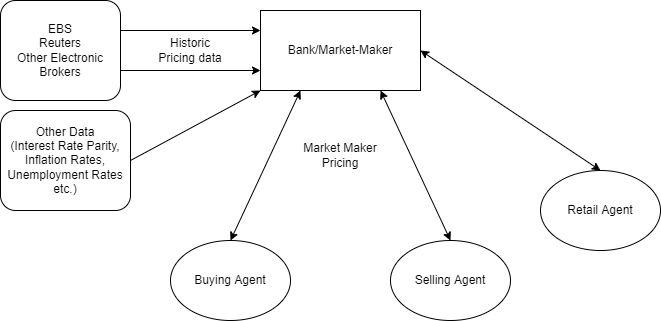
\includegraphics[scale=0.6]{model_architecture.png}
  \caption{Agent Based Model Design}
  \label{fig:model}
\end{figure}


The mechanism in which the market-maker will determine an exchange rate depends on a number of factors. Each market-maker in reality will have a different way of calculating this rate and will apply their own margins accordingly to service their clients. For this model, all market makers will use the same method to determine the exchange rate, but will be given some variance factors that will make each bank in the model have different rates at different times. The change in exchange rate for the model will be made up of the interest rate parity, the money supply of the given currency and the inflation rates and unemployment data for each country. This can be given as the following: $\Delta R_t = f(i, m, x) + \mu _t$ where $\Delta R_t$ is the change in exchange rate, $f$ is a function that is applied to the given data to transform it into the given exchange rate for a market-maker. $i$ is the interest rate parity, $m$ is the money supply, $x$ is the other macro-economic factors such as unemployment data, inflation rate, etc. $\mu _t$ is the residual noise term to lead to a stable model that reaches an equilibrium quickly. \cite{delage2011multi}


